\chapter{State of the art}\label{A:stateOfTheArt}

This chapter aims to provide a vision of how the audio-visual media production sector has been, and still is, carrying out IP convergence. 

Moreover, this chapter will be focused on the topics related to media production over an IP related environment and, specifically, the ones related on this project study and proposal.

\section{Audio-visual media content production}

As briefly as possible, this section aims to summarise the evolution of the IP convergence itself and how technologies are evolving to carry out such transformation at audio-visual media content production level.

This subsection is organized by enumerating potential technologies and standards by following the OSI stack from the bottom layer.

\subsection{Physical and Data link layers}

Ethernet was standardised in 1983 and since then the standard has been increasing its speed rate from the initial 10 Mbps to 100 Gbps (foreseen 400 Gbps by IEEE P802.3bs Task Force), with currently easily affordable 10 Gbps and 40 Gbps interfaces. These rates seem to be enough to accommodate current broadcast formats (e.g.: HD at ~1.5 Gbps, 3G at ~3 Gbps and UHD at ~12 Gbps) and further innovations because of the nature of the packet technologies make them completely agnostic to the upper formats and indeed transparent for future formats in contrast with current media transport technologies which are completely bounded with the transported formats (i.e.: standard cable video formats used over broadcast environments). On another hand, Ethernet hasn't got any timing awareness or QoS assurance, so it makes difficult to accommodate current operation workflows over this technology. Nevertheless, because Ethernet is widely used in the IT industry, its use, as COTS switches, have motivated studies about the use of these switches in the broadcast industry deployments to validate specific necessary features as the latency deviation or packet loss. (REFERENCE: TEST LINK3)

At the same level, to address some of the inherent Ethernet limitations, Audio Video Bridging (AVB) appeared in 2011 which is a set of standard extensions to the Ethernet IEEE 802.1 focusing on timing and QoS guarantee within local area networks. Its approach is a plug-and-play platform to ease transition from current transport technologies to the newer ones using the same workflows, but the current version is still limited to local premises and limited topologies. Since November 2012, because more varied industry sectors joined the task group, a more general name, Time Sensitive Networks (TSN), was created to carry on with the new developments.

On another hand, the emergence of the SDN paradigm (--REFERENCE--), separating the control and forwarding plane besides creating northbound interfaces to interact with external applications enables new flexible and customised network operations and deployments. There are a lot of foreseen benefits from this approach but to be fully capable of support all type of streams some extensions should appear, such as a specific extension which has been released by the ONF to address timing restrictions known as OpenFlow Time Extension to OpenFlow 1.3.x ext340 (--REFERENCE--).

Furthermore, the Telecom Industry introduced the NFV concept (--REFERENCE--) in 2012 to enable the shifting from the hardware-centric approach to the software-centric one. In spite of not being thought for
broadcasting issues, this parading provides an amazing flexibility to bring up new deployments, enhance current workflows and create future ones.

Related to above statements, the recent advances in chip designs, by industry leaders, such as Intel, Broadcom, Xilinx, Altera, \ldots, have eased a strong movement towards consolidation of complex functions (such as encoding, transcoding, conversion, \ldots ) into a single device, instead
several disparate platforms. Additionally, these hardware advances implied the chance of using software-centric frameworks, which provide for greater flexibility and customization from a business standpoint. Coupled together, these advances will enable a broader adoption of upcoming media technologies, at a reduced cost, without compromise on quality, flexibility and or capability. The disruptive nature of such advances can be readily seen in the mobile telephony market, such as the entry of open source mobile phone software (e.g.: Google’s Android OS) which when couple with low cost but powerful chipsets, has democratised the market, allowing millions of low income countries access to mobile phones and with it the Internet.

In parallel, regarding the specific timing and synchronising requirements of live media production, the standard IEEE 1588-2008 (--REFERENCE--), commonly known as PTPv2(--REFERENCE--), appeared covering several profiles to be used through several network environments. For instance, SMPTE(--REFERENCE--) published a draft profile SMPTE ST 2059 (1 and 2) (--REFERENCE--)defining a reference alignment to SMPTE epoch and there are studies analysing the application of PTP to broadcast environments under different circumstances (check this demo LINK4 --> Check also annex with ieee presentation!).

\subsection{Network and Transport layers}

On the network layer, IP is the de facto standard and within its protocol suite there are some solutions which help to transport media content efficiently. For instance, IP supports multicast paradigm operation using widely supported routing protocols (DVMRP, PIM, IGMP, \ldots) but the
computational and scalable complexity of these protocols tends to complex and limited deployments.

Regarding QoS, IP has a mechanism known as ToS/DSCP which marks the packets (in the header) along their way to help mappings with lower-layer protocols (as Ethernet or MPLS) to implement QoS at the buffer level. Furthermore, IP networks have been evolving its own architectures from
traditional hierarchic ones to flatter ones, such as the leaf-and-spine, used in most of the big data centre deployments nowadays by facilitating horizontal data movement which is useful for heavy load transactions between same level hosts.

On the transport layer, UDP has been preferred over TCP for real-time transport because of its connectionless avoiding unnecessary retransmission for live streams. A basic extension, RTP, which its most
deployed version is RFC 3550, was introduced to transport audio and media services using a timestamp field together with the protocol for control purposes (RTCP). Recently, new extensions have appeared introducing new header options to support the adoption of services related to media production workflows. Concretely, RTP and RTCP have been proposed to accommodate media specific info over IP, answering to specific challenges.

\subsection{Session, Presentation and Application layers}

Encapsulation audio (AES67-2013) and video (SMPTE 2022-6) standards have appeared (2012-2013) to transport high-quality media signals over IP Networks, but specially in the audio field a broad spectrum of proprietary solutions exist such as Dante, RAVENNA or Livewire (-- FOOTNOTE??--).

On the video side, SMPTE 2022-6 is focused on mapping SDI and HDSDI (opposite to raw video, audio and metadata mapping, known as essence mapping) within IP packets and further specific solutions for manage packet loss recovery using FEC (SMPTE 2022-5) and a seamless protection
system (SMPTE 2022-7).

In the middle of 2014, the Video Services Forum (VSF) has formed a new group (SVIP) looking at new encapsulation mechanisms for audio, video and ancillary data into IP without using SDI framing (raw data) to develop or recommend a standard for video over IP without SDI encapsulation.
They aim to study and document the requirements for video over IP/Ethernet within plant (video, audio, ancillary data, bundles, timing, sequencing, identities, and latency), to research current and proposed solutions to report on gaps between requirements and existing solutions (especially regarding existing SMPTE 2022 Standards) and finally to propose scope for follow on activity if required.

On another hand, the wide adoption of low-delay encoding (e.g.: JPEG2K, AVC, AVCi, VC-2) for high- quality video stream could represent a new opportunity to reduce the bandwidth consumption in several scenarios. Likewise, high-compression mechanism as MPEG4 H264 or HEVC could be
useful to transport media content through very limited network resources scenarios (as Internet or cloud-based systems).

Moreover, specific efforts have risen to arrange specific challenges such as a networked media interface by Sony to carry a virtually lossless UHD/4K (12 Gbps non-compressed) over a single 10 GBE interface, limited proofs of concept or specific implementations facing the switching-point issue. All of these are a useful starting point for future enhancements towards a global operational framework. (RESOURCES/REFERENCES??? LINK5)

Another important issue is the automation of the system to enhance flexibility for deployment set-up and maintenance. Here, some solutions as Zero-configuration networking (-- REFERENCE - LINK6 ) could contribute using well-known protocols as DHCP or DNS-SD to enable auto-configuration and streaming announcement, but to be implemented in an operational scenario a common approach should be
defined.

In the media plane, protocols as RTSP for end-to-end session control or SDP for service description provide capabilities for the stream management. Complementary, media wrappers aim to gather different types of programme media and associated information, as well as generically identify this information. Different media wrapper formats are in use at this time (e.g.: MXF LINK7), but, for the media industry, it is important that the wrappers have characteristics like openness, extensibility, performance \ldots The MXF (a SMPTE standard) is a “container” format which supports a number of different streams of coded based, encoded in any of a variety of video and audio compression formats, together with a metadata wrapper which describes the material contained within the MXF file enable interoperability
between different platforms. Also DDS (a machine-to-machines middleware standard from OMG --REFERENCE--) could be used to enable interoperable media exchange between actors. At the same time, EBU has launched the FIMS (Framework for Interoperable Media Services --REFERENCE--) which intends to answer to different interoperability issues between SOA proprietary systems by defining an open, consensual framework with standardised interfaces.

Regarding the measurement of media transport over IP, VSF published in 2006 a document (RVOIM LINK8 ) to define the recommended metrics for Video over IP transport. The aim of the document is help in the monitoring, troubleshooting, equipment performance compliance to standards and specifications, verifying and measuring the delivered services statistics and equipment analysis and debug, but basically with a distribution approach, not focused on live production as the current project aims.

As could be inferred from the above statements, there are no current common approach to solve the whole challenge yet and to face this issue some initiatives have appeared lately. Many outstanding research initiatives are on the way but an interesting one was carried out by the BBC (--REFERENCE - LINK9) which tried to provide an operational framework for a live studio within their environment.

Likewise, in 2013 SMPTE, VSF and EBU created the JT-NM task force (JTNM) to drive the broadcasting industry towards a full IP adoption by providing guidelines to enable a successful migration. Currently, the JT-NM is working to develop a reference architecture (phase 2) to help all involved layers to agree on all cross issues whereas defining specific requirements over concrete use cases to uncover missing definitions to address the general scenario (--REFERENCE -- LINK10).

\section{Migration to cloud}

This section is a continuation of the previous one but showing how other topics related to IP convergence are giving new chances to improve audio-visual media production at any possible production environment, concretely within the cloud concept. 

\subsection{Cloud computing}

Cloud computing describes the delivery of shared computing resources (software and/or data) on demand through the Internet and its benefits can be foreseen as it is defined by the NIST recommendations (--SEE ANNEX X OR REFERENCE--). So for reasons of flexibility, security, data protection, agility and cost, many organisations are embracing cloud computing. 

Nowadays, cloud computing is defined by three fundamental models that are organized through application/service, platform and infrastructure layers.

\begin{figure}[htb]
\begin{center}
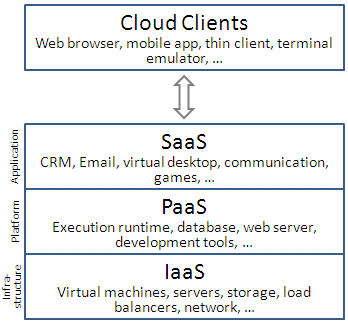
\includegraphics[width=0.35\textwidth]{./images/Cloud_computing_layers.png}
\caption{Cloud computing layers}
\label{F:cloudComputingLayers}
\end{center}
\end{figure}

Moreover, there are different deployment models depending on the "product" behind and which are the resources from the entity that is offering or using such product. Main deployment models might be:

\begin{itemize}
\item Public: when applications/services run over a network that is open for public use, which may be free. The fact of being public/opened implies much more complexity in terms of security issues.
\item Private: when infrastructure is operated solely for a single organization, whether managed internally or by a third-party, and hosted either internally or externally. This cloud type might be similar in terms of architecture design from the public one.
\item Hybrid: when a composition of two or more clouds (private or public ones) are treated as distinct entities but are bound together, offering the benefits of multiple deployment models. Hybrid cloud allows to extend either the capacity or the capability of a cloud service, by aggregation, integration or customization with another cloud service.
\end{itemize}

To point out that high-performance computing (e.g.: GPU based clouds --REFERENCE--) and software-defined networking (SDN) could shape where cloud is evolving and it could improve solutions to current cloud issues such as security (-- REFERENCE - National Security Agency and PRISM scandal), processing performance, full processing chaing control through specific SLAs, \ldots

In many terms, the cloud concept is key solution to help media producers create better content more quickly and there are lots of examples to focus on, but lets introduce the ones that tends to flexible and scalable ways to access the benefits that cloud computing brings to media production:

\begin{itemize}
\item Low-cost initial expenditures \hfill 

Media production tends to require an enormous initial investment in technology infrastructure and the technical staff to manage it. In that sense, cloud computing technology is that the creative industries are alleviated of the need to invest heavily in technology that would rapidly become obsolete. Cloud computing allows the media production industry to provision only the technology they need, when they need it, avoiding excessive CAPEX.

\item Cost forecasting\hfill 

Infrastructure as a Service (Iaas) prices are predictable and granularly treated. It allows prediction on a per project basis with detailed cost analysis precision. As done by many IaaS providers (e.g..: Amazon, Woowza, \ldots), each resource used in a media production workflow is metered, and companies pay only for what they use.

\item Dynamic infrastructure deployment \hfill 

Cloud computing helps production entities take advantage by the on demand basis applied deployments. Media production companies can quickly provision servers to meet the demands of specific projects and shut them down when they are no longer needed.
\end{itemize}

Moreover, cloud computing can improve media production at many different media services requirements planes such as:

\begin{itemize}
\item Media asset management
\item Granular costs measurement
\item Cloud transcoding
\item High-speed file transfer
\item Automated content verification
\item Elastic deployment
\item Real-time and full monitoring
\item Video quality control
\end{itemize}

And, expected overall outcomes might be:

\begin{itemize}
\item Increased performance
\item Lowered costs
\item Improved cross collaboration
\end{itemize}

As a corollary, figure \ref{F:cloudComputingLayers} describes generic cloud computing layers, but it also refers to this project's topics in order. These are virtualization, monitoring and media/coding.

\subsection{Virtualization}

Virtualization, under computing environments, means creating a virtual version of any possible piece of actual hardware or software so that we can use system resources effectively. Besides hardware and desktop virtualization, which are the most known commercial concepts, it can be explained and organized in two different concepts:

(TO EXPLAIN EACH SUBITEM)
\begin{itemize}
\item Types
\begin{itemize}
\item Data virtualization
\item Memory virtualization
\item Network virtualization
\item Storage virtualization
\item Security virtualization
\end{itemize}
\item Levels
\begin{itemize}
\item Application virtualization
\item Environment virtualization
\item Operating System (OS) virtualization
\item Networking virtualization
\end{itemize}
\end{itemize}

Cloud computing is usually strongly related and implemented with different kinds of virtualization. Many virtualization methods are commonly implemented at datacenters where platforms and services are going to be deployed over different infrastructure architectures. Nevertheless, deploying virtualization at data centers doesn’t automatically mean running over a cloud and it’s possible to deploy clouds without virtualization.

As well as cloud computing concept started to be widely used from 2000's, virtualization  technologies can be traced back to the 1960’s such as virtual desktops, and others can only be traced back a few years, such as virtualized applications.

INTERESTS AND COMPARISONS (TENDENCES) -> TALK ABOUT KVM AND LXC
Containers represent one of the leading trends in computing today. With companies such as Docker, CoreOS, ClusterHQ joining industry giants like IBM, Red Hat, MIcrosoft and others in the rush to speed up the pace of container adoption. A recent study by DevOps.com and ClusterHQ showed that over 90% of organizations have either looked at or plan to look at containers in the near future.



FINALLY:
Virtualization can increase IT agility, flexibility, and scalability while creating significant cost savings. Workloads get deployed faster, performance and availability increases and operations become automated, resulting in IT that's simpler to manage and less costly to own and operate.
Reduce capital and operating costs.
Deliver high application availability.
Minimize or eliminate downtime.
Increase IT productivity, efficiency, agility and responsiveness.
Speed and simplify application and resource provisioning.
Support business continuity and disaster recovery.
Enable centralized management.
Build a true Software-Defined Data Center.




\subsection{Monitoring}

monitoring: mrtg (tobias oeticker - rrdb), cactix,...

\subsection{Media streaming}

CHECK wikipedia -> advanced television system committee standards

transcoding, codecs, codification (nowadays), 

\section{LiveMediaStreamer (LMS) framework}







